\documentclass[a4paper]{article}

\usepackage[english,ngerman]{babel}
\usepackage[T1]{fontenc}
\usepackage[utf8]{inputenc}
\usepackage{lmodern}
\usepackage{amsmath}
\usepackage{subcaption}
\usepackage{icomma}
\usepackage{tikz}
\usetikzlibrary{shapes,arrows,positioning}
\renewcommand{\u}[1]{\;\mathrm{#1}}
\newcommand{\uf}[1]{\;\mathrm{#1}}
\useshorthands*{"}
\addto\extrasenglish{\languageshorthands{ngerman}}

\begin{document}

\tikzstyle{block} = [draw, rectangle, minimum height=2em, minimum width=2em]
\tikzstyle{sum} = [draw, circle]
\tikzstyle{input} = [coordinate]
\tikzstyle{output} = [coordinate]
\tikzstyle{pinstyle} = [pin edge={to-,thin,black}]

\author{Oliver Arend}
\title{Developing an appropriate PID controller for RTVC using a Kalman filter for state estimation}
\date{2017--12}
\maketitle

\section{Model development}

\begin{figure}[b]
\begin{center}
\begin{tikzpicture}[auto,node distance=2cm,>=latex']
    \node [input] (input) {};
    \node [sum, right of=input] (sum_x) {};
    \node [block, right of=sum_x] (PID) {PID};
    \node [block, right of=PID] (rocket) {system};
    \node [output, right of=rocket] (output) {};
    
    \draw [->] (input) -- node {$x_0$} node [pos=0.9] {$+$} (sum_x);
    \draw [->] (sum_x) -- node {$e$} (PID);
    \draw [->] (PID) -- node {$u$} (rocket);
    \draw [->] (rocket) -- node [near start] {$x$} (output);
    
    \draw node at (7,0) {\textbullet};
    \draw [->] (7,0) |- (2, -1) -| node [pos=0.90] {$-$} (sum_x);
    \draw node at (6,1) {process noise $w$};
    \draw [->] (6,0.8) -| (rocket);
\end{tikzpicture}
\end{center}
\caption{Simple system including a PID controller} \label{fig:simple}
\end{figure}

\begin{figure}[t]
\begin{center}
\begin{tikzpicture}[auto,node distance=2cm,>=latex']
    \node [input] (input) {};
    \node [sum, right of=input] (sum_x) {};
    \node [block, right of=sum_x] (PID) {PID};
    \node [block, right of=PID] (servo) {servo};
    \node [block, right of=servo] (rocket) {rocket};
    \node [output, right of=rocket] (output) {};
    
    \draw [->] (input) -- node {$x_0$} node [pos=0.9] {$+$} (sum_x);
    \draw [->] (sum_x) -- node {$e$} (PID);
    \draw [->] (PID) -- node {$u$} (servo);
    \draw [->] (servo) -- node {$M$} (rocket);
    \draw [->] (rocket) -- node [near start] {$x$} (output);
    
    \draw node at (9,0) {\textbullet};
    \draw [->] (9,0) |- (2, -1) -| node [pos=0.90] {$-$} (sum_x);
    \draw node at (8,1) {process noise $w$};
    \draw [->] (8,0.8) -| (rocket);
\end{tikzpicture}
\end{center}
\caption{Separating complete system into servo and rocket subsystems} \label{fig:subsystems}
\end{figure}

Typically, a system is designed to operate in a certain state described by one or more state variables $x$. The desired state is described by the setpoint $x_0$, and the difference between these two values is the error $e$. A controller is then designed to give an input $u$ to the system such that the error is minimized. Such a system is shown in figure \ref{fig:simple}. The behavior of the system is not completely deterministic since some unknown process noise $w$ is acting on the system, hence the need for a controller.

In our case, the system is basically comprised of two subsystems, considering one axis of yaw/pitch:
\begin{enumerate}
\item The servo being controlled by the controller through the command $u$ and accordingly exerting a torque $M$ on
\item the rocket, which has certain known characteristics such as its moment of inertia $J$, but is also subject to unknown disturbances (process noise) from wind or lack of detail in the model.
\end{enumerate}
Such a system is shown in figure \ref{fig:subsystems}.

\section{PID controller design} \label{PID}

\begin{figure}[b!]
\begin{center}
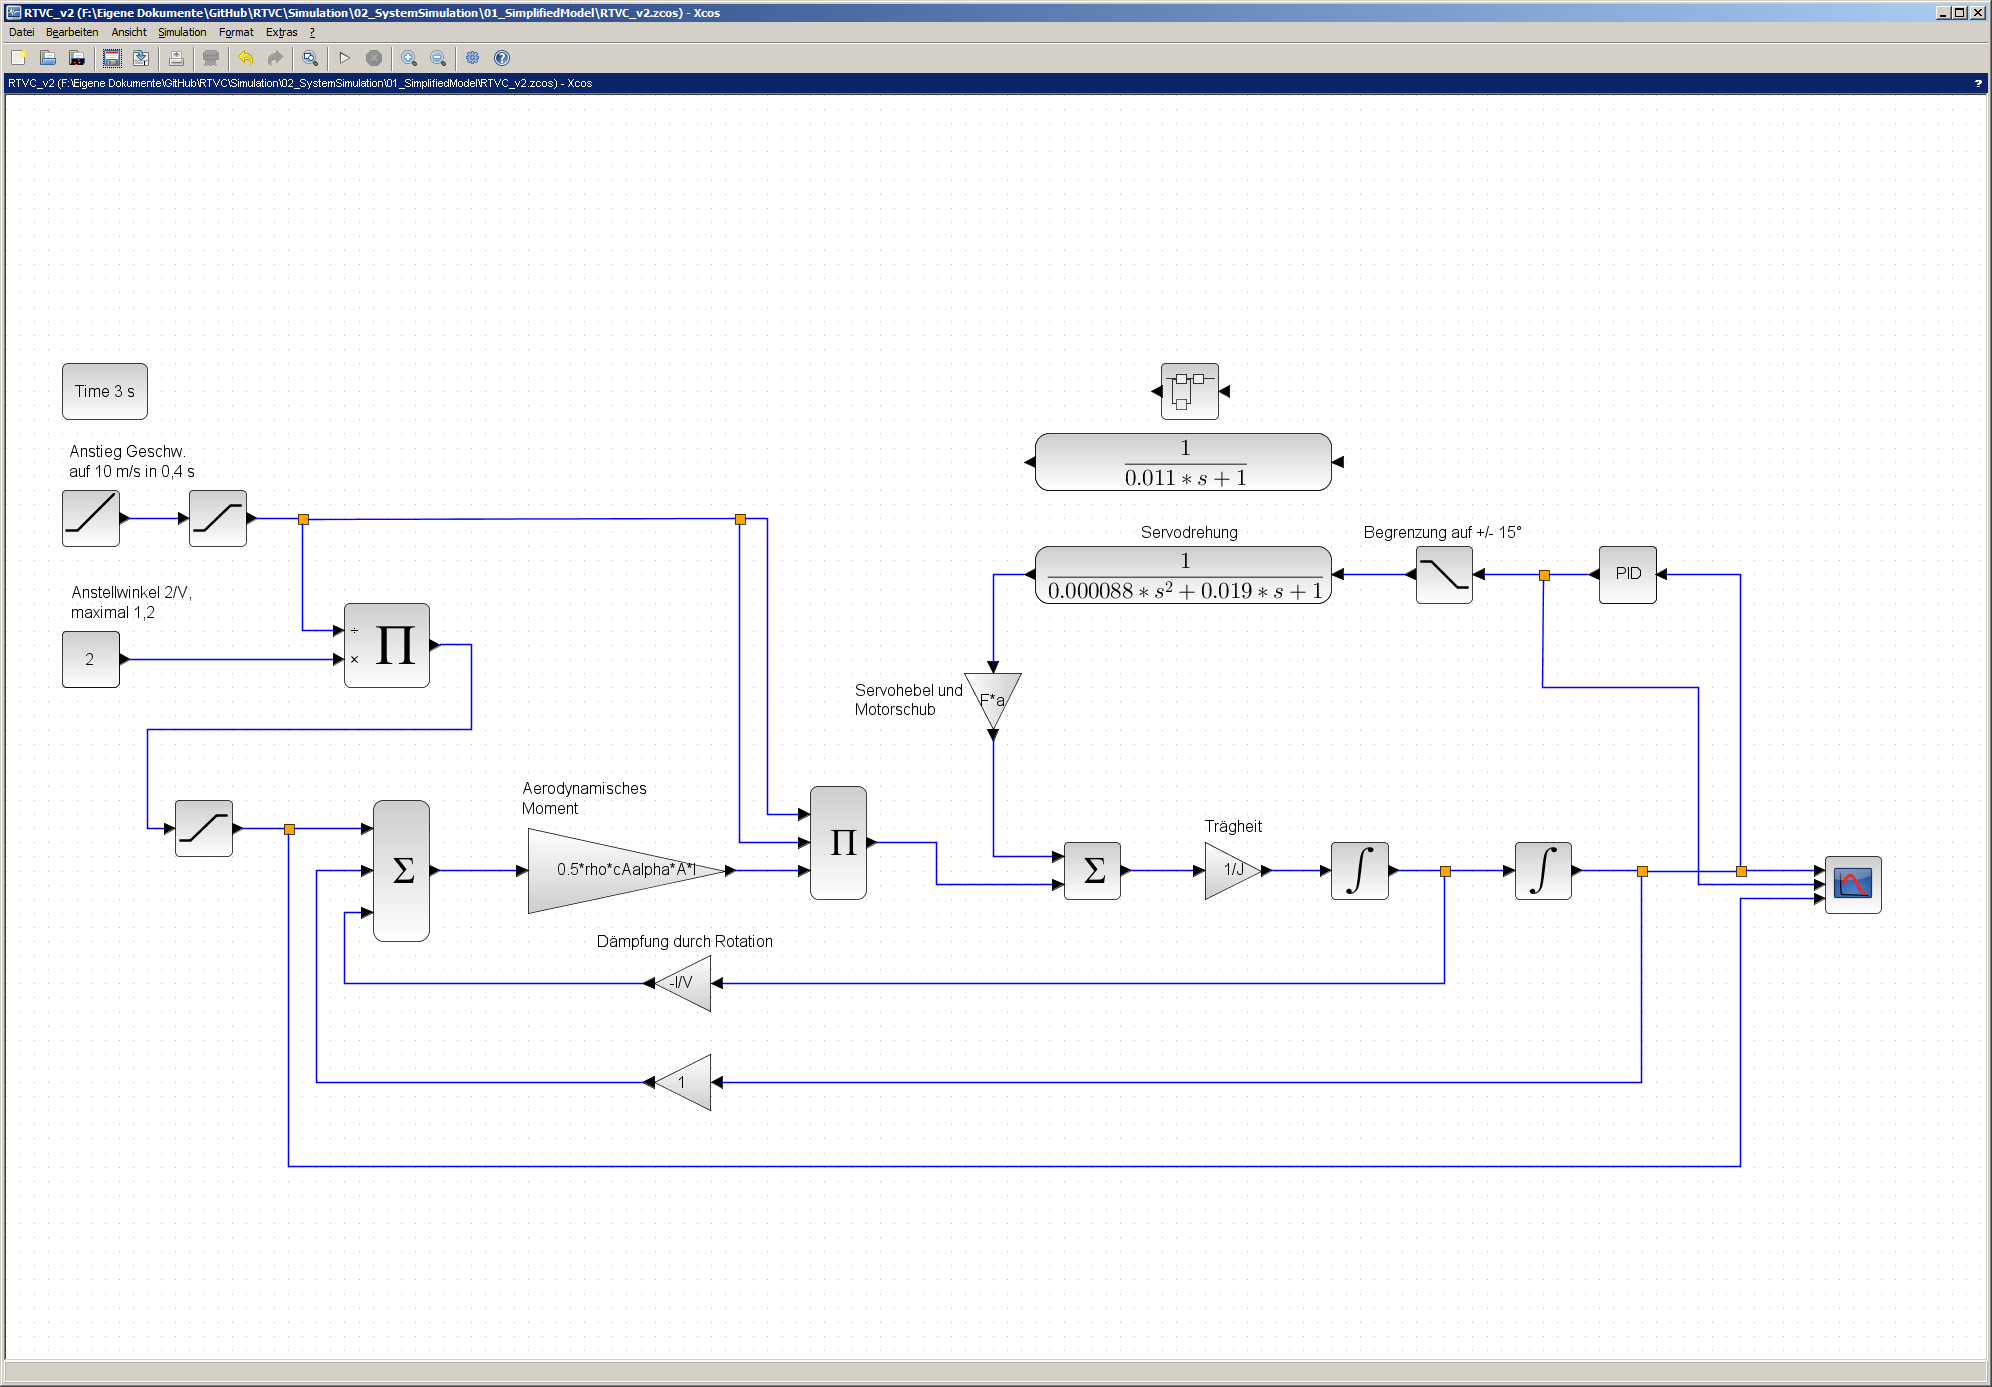
\includegraphics[width=120mm]{model.png}
\end{center}
\caption{\textsc{scilab} model used for PID controller design} \label{fig:scilabmodel}
\end{figure}

A PID controller is described by three values $K_P$, $K_I$ and $K_D$ determining the output $u$ as a function of the error $e$ (in continuous form): \begin{equation}u(t) = K_P e(t) + K_I \int^t_0 e(t) dt + K_D \frac{de(t)}{dt}\end{equation}i. e. it takes into account
\begin{itemize}
\item the current magnitude of the error $e(t)$ at time $t$ and producing a proportional output with a proportionality factor $K_P$ -- the larger the error, the larger the corrective action. This in turn means that the error would never disappear entirely, hence the need for an
\item integral output. If the error accumulates over time $\int e(t) dt$ the corrective action will be greater, with a factor of $K_I$.
\item The last part is an output proportional to the current rate of change of the error $\frac{de(t)}{dt}$ with a factor of $K_D$; if it changes more quickly, the corrective action will need to be greater.
\end{itemize}
The values $K_P$, $K_I$ and $K_D$ were determined empirically using the \textsc{scilab} model shown in figure \ref{fig:scilabmodel}. It includes an environment where airspeed $V$ increases linearly from $0$ to $10\u{m/s}$ in $0.4\u{s}$ with an angle of attack $\alpha = \min \left(1.2, \frac{2\u{m/s}}{V} \right)\u{rad}$. Through this angle of attack the rocket, in particular the nosecone, creates an aerodynamic torque \begin{equation}M_{aero} = \frac{1}{2} \rho V^2 c_{A_{\alpha}} \alpha A \ell \end{equation} around its yaw/pitch axis. Air density is assumed standard conditions $\rho = 1.225 \u{kg/m^3}$, the coefficient of lift gradient is $c_{A_{\alpha}} = 2$ for nosecones, the reference section is $A = 0.00353\u{m^2}$ for a rocket diameter of $67\u{mm}$ and the moment arm $\ell = 0.1\u{m}$ as the distance between the nosecone's center of pressure and the rocket's center of gravity. The torque translates into an angular acceleration $\ddot{\gamma} = \frac{M_{aero}}{J}$ of the rocket's path $\gamma$ with the rocket's inertia $J=8.1 \cdot 10^{-4}\u{kg\,m^2}$, integrated twice to yield path angular velocity $\dot{\gamma}$ and path angle, respectively. The angular velocity results in an effective reduction of the angle of attack through moment arm and velocity $\Delta \alpha = - \frac{\ell}{V} \dot{\gamma}$.

The PID controller factors yielding a satisfactory behavior of the rocket as described above are \begin{eqnarray}
K_P & = & -5 \\
K_I & = & -5 \\
K_D & = & -1
\end{eqnarray}
with the output as the setpoint for a servo motor controlling the angle $\varphi$ (in the same unit as the path angle of the rocket) of the rocket motor relative to the longitudinal axis of the rocket. 

The servo of course does not move instantaneously, but the reaction to a change in the setpoint is very similar to a PT2 element with the transfer function \begin{equation}G(s) = \frac{1}{0.000088 s^2 + 0.019 s + 1}\end{equation}corresponding to the two time constants $T_1 = 0.008\u{s}$ and $T_2=0.019\u{s}$. This behavior can also be described in the state space as \begin{equation}\dot{X} = \begin{pmatrix}0 & 1 \\ -11364 & -216\end{pmatrix} X + \begin{pmatrix}0 \\ 11364\end{pmatrix} u\label{eq:servo}\end{equation} with $X=\begin{pmatrix}\varphi \\ \dot{\varphi}\end{pmatrix}$ and $u$ the servo angle setpoint.

\section{Kalman filter design}

\begin{figure}[t]
\begin{center}
\begin{tikzpicture}[auto,node distance=2cm,>=latex']
%    \draw[help lines] (0,-2) grid (8,3);
    \node [input] (input) {};
    \node [block, minimum width=3cm, right of=input, align=center] at (0.5,0) (system) {system \\ $\dot{X} = AX+w$ \\ $Y = CX$};
    \node [sum, right=1.3cm of system] (sum_y) {};
    \node [block, right of=sum_y, align=center] (kalman) {Kalman\\filter};
    \node [output, right of=kalman] (output) {};
    
    \draw [->] (system) -- node {$Y$} node[pos=0.8] {$+$} (sum_y);
    \draw [->] (sum_y) -- node {$\tilde{Y}$} (kalman);

    \draw node at (2.5,1.5) {process noise $w$};
    \draw [->] (2.5,1.3) -| (system);

    \draw node at (5.5,1.5) {signal noise $v$};
    \draw [->] (5.5,1.3) -| node[pos=0.9] {$+$} (sum_y);
    
    \draw [->] (kalman) -- node {$\hat{X}$} (output);
\end{tikzpicture}
\end{center}
\caption{Typical Kalman filter approach} \label{fig:Kalman}
\end{figure}

A Kalman filter can be used to estimate the current state of a system by using knowledge about the behavior of the system, the quality of the measurement and of course the measurements itself. Based on this, for every timestep the filter will first predict the current state of the system and then correct this estimate based on a measurement and the prediction's certainty.
The behavior of a system can be described as \begin{eqnarray}\dot{X} &=& A X + B U + w \\
Z &=& C X + v\end{eqnarray} with the state of the system $X$, commands $U$, process noise $w$ (which includes uncertainties about the behavior of the system and unknown outside influences), measurements $Z$, measurement noise $v$ (which is more or less known) and matrices $A$, $B$, $C$ and $D$ describing the relationships between these. From a time-discrete perspective, this can also be written as \begin{eqnarray}X_i &=& A X_{i-1} + B U_i + w_{i-1} \\
Z_i &=& H X_i + v_i\end{eqnarray}The Kalman filter uses this information to estimate the system's state using two steps:\begin{description}
\item[Prediction]In this step the current state will be predicted from the last estimate according to the system's behavior \begin{eqnarray}\hat{X}^-_i &=& A \hat{X}_{i-1} + B U_i \\
P^-_i &=& A P_{i-1} A + Q\end{eqnarray} with the system error covariance matrix $Q$ and the error covariance $P$. $Q$ is unknown and can only be estimated. $P$ can be initialized to the identity matrix.
\item[Correction]The predicted state will now be corrected according to the measured values describing (part of) the state:\begin{eqnarray}K_i &=& P^-_i H^T(H P^-_i  H^T+R)^{-1} \\
\hat{X}_i &=& \hat{X}^-_i + K_i(Z_i - H\hat{X}^-_i) \\
P_i &=& (I - K_i H)P^-_i\end{eqnarray}
\end{description} A rough sketch of how a Kalman filter estimates the system's state from its measurement output(s) is shown in figure \ref{fig:Kalman}.

\subsection{Model rocket apogee detection}

As a simple first example, the Kalman filter is applied to a model rocket flying up and whose apogee should be detected. The state of the rocket can be described as \begin{equation}X = \begin{pmatrix}h\\v\\a\end{pmatrix}\end{equation}with altitude $h$, (vertical) velocity $v$ and (vertical) acceleration $a$. The evolution from one state to the next is done through simple integration with a time constant $\Delta t$. No commands $U$ are imparted to the rocket, and the measurement is simply the altitude $h$, with a measurement noise covariance of $R=0.25$. The system variables are in basic SI units (meters and seconds). The relevant matrices are thus \begin{align}A&=\begin{pmatrix}1 & \Delta t & 0 \\ 0 & 1 & \Delta t \\ 0 & 0 & 1\end{pmatrix}, &B&=0 \\ C&=\begin{pmatrix}1 & 0 & 0\end{pmatrix}, &D&=0\end{align}

\begin{figure}[b]
\centering
\begin{subfigure}[t]{0.48\textwidth}
\centering
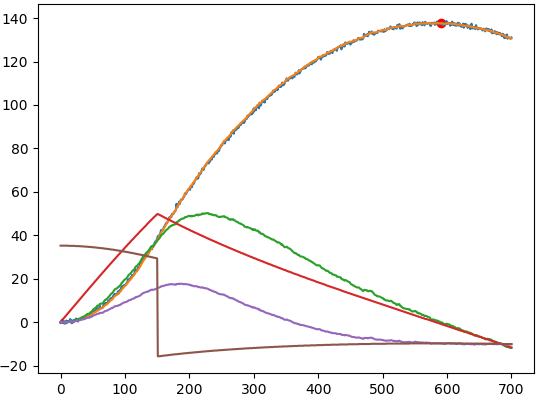
\includegraphics[width=\textwidth]{kalman_altitude.png}
\caption{From altitude measurement only} \label{fig:altitude}
\end{subfigure}
\begin{subfigure}[t]{0.48\textwidth}
\centering
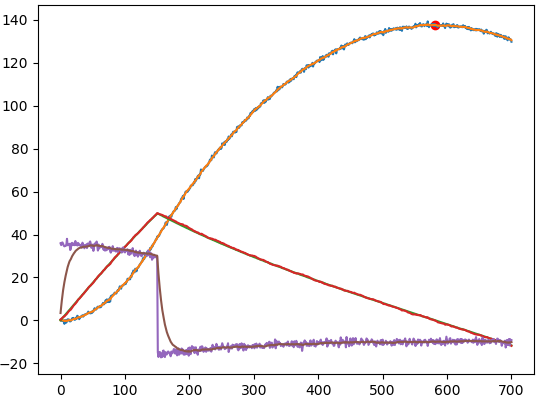
\includegraphics[width=\textwidth]{kalman_altitude_accel.png}
\caption{From both altitude and acceleration measurements} \label{fig:altitude_accel}
\end{subfigure}
\caption{Estimating altitude and apogee}
\end{figure}

Data was created with a time increment of $0.01\u{s}$ from a rocket flight simulation, with additional noise added to the altitude measurement. The results from \texttt{kal""man\_""rocket""flight\_""alti""tude"".py} are shown in figure \ref{fig:altitude}. The measured altitude is shown in light blue, and its estimate in orange. The filter reduces the noisiness quite a bit, but does not completely eliminate it ($Q=0.01 I$ was chosen). Velocity (true red, estimate green) and acceleration (true dark purple, estimate light purple) were also estimated, but do not match the true values closely. Only apogee detection, with $v=0$, would work reliably.

Results can be improved considerably using an accelerometer, hence changing the measurement matrix to \begin{equation}C=\begin{pmatrix}1 & 0 & 0 \\ 0 & 0 & 1\end{pmatrix}\end{equation} and the measurement covariance matrix to \begin{equation}R=\begin{pmatrix}0.25 & 0 \\ 0 & 1\end{pmatrix},\end{equation} assuming independent error. The results from \texttt{kal""man\_""rocket""flight\_""alti""tude\_""accel"".py} are shown in figure \ref{fig:altitude_accel}. Velocity matches very well, while the acceleration estimate takes some time to converge to the true value.

\subsection{Simple model rocket attitude control}

The actual application of the Kalman filter towards an active control of the rocket's attitude involves measuring the rocket's angular velocity and estimating its path angle, which should be kept at or very near 0. It is simplified to a single pitch/yaw axis, because both axes can be regarded as independent of each other.

A simple model would only involve a state representing the rocket's attitude and its evolution \begin{equation}X=\begin{pmatrix}\gamma \\ \dot{\gamma} \\ \ddot{\gamma} \end{pmatrix}\end{equation} with the path angle $\gamma$ and its time derivatives. Reusing the \textsc{scilab} model to design the PID controller (see section \ref{PID}), noisy data representing the angular velocity $\dot{\gamma}$ is created. For comparison, clean data for path angle $\gamma$, angular velocity and the corrective command to the servo $u$ is also exported.

\begin{figure}[t]
\centering
\begin{subfigure}[t]{0.48\textwidth}
\centering
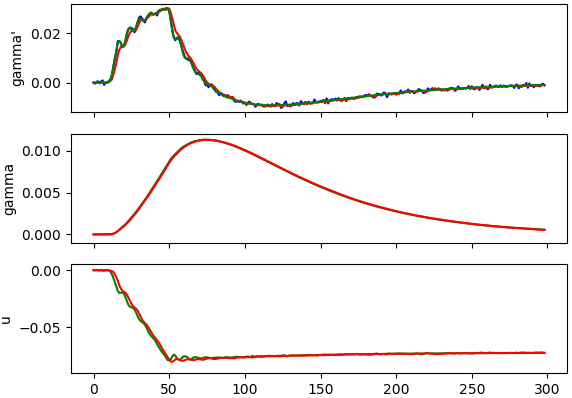
\includegraphics[width=\textwidth]{kalman_attitude_B0.png}
\caption{Ignoring $u$ ($B=0$)} \label{fig:simple_attitude_B0}
\end{subfigure}
\begin{subfigure}[t]{0.48\textwidth}
\centering
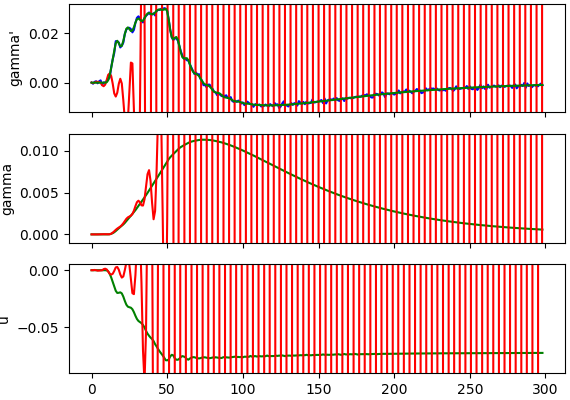
\includegraphics[width=\textwidth]{kalman_attitude_Bdirect.png} 
\caption{Translating $u$ directly to angular acceleration} \label{fig:simple_attitude_Bdirect}
\end{subfigure}
\caption{Estimating the rocket's attitude using only path angle and derivatives as state} \label{fig:simple_attitude}
\end{figure}

Two approaches were used: \begin{itemize}
\item completely ignoring the servo command in the prediction, such that \begin{equation}A = \begin{pmatrix}1 & \Delta t & 0 \\ 0 & 1 & \Delta t \\ 0 & 0 & 1\end{pmatrix}, \quad B = \begin{pmatrix}0 \\ 0 \\ 0\end{pmatrix}\end{equation}
\item and directly translating the setpoint of the servo $u$ to an angular acceleration such that \begin{equation}A = \begin{pmatrix}1 & \Delta t & 0 \\ 0 & 1 & \Delta t \\ 0 & 0 & 1\end{pmatrix}, \quad B = \begin{pmatrix}0 \\ 0 \\ \frac{Fa}{J}\end{pmatrix}\end{equation}with the motor's thrust $F$, the moment arm of the motor $a$ and the rocket's angular inertia $J$.\end{itemize}
The results of both approaches are shown in figure \ref{fig:simple_attitude}. Obviously the approach considering the torque applied by the rotating motor leads to a divergent estimate, see figure \ref{fig:simple_attitude_Bdirect}, since the servo does not actually move that fast -- the timestep in the simulation is $0.01\u{s}$, whereas the time constant of the servo is about $0.019\u{s}$. Ignoring $u$, as shown in figure \ref{fig:simple_attitude_B0}, leads to a decent estimate of the path angle $\gamma$, but some error and phase offset in angular velocity $\dot{\gamma}$ and the servo command $u$.

\subsection{Complex attitude estimate and control}

\begin{figure}[t]
\hspace{-10mm}
\begin{tikzpicture}[auto,node distance=2cm,>=latex']
    \node [input] (input) {};
    \node [sum, right of=input] (sum_x) {};
    \node [block, right of=sum_x] (PID) {PID};
    \node [block, right of=PID] (servo) {servo};
    \node [block, right of=servo] (rocket) {rocket};
    \node [sum, right of=rocket] (sum_y) {};
    \node [block, minimum height=1.5cm, minimum width=2cm, right of=sum_y, align=center] (kalman) {Kalman\\filter};
    \node [output, right of=kalman] (output) {};
    
    \draw [->] (input) -- node {$x_0$} node [pos=0.9] {$+$} (sum_x);
    \draw [->] (sum_x) -- node {$\hat{e}$} (PID);
    \draw [->] (PID) -- node {$u$} (servo);
    \draw [->] (servo) -- node {$M$} (rocket);
    \draw [->] (rocket) -- node {$Y$} node[pos=0.8] {$+$} (sum_y);
    \draw [->] (sum_y) -- node {$\tilde{Y}$} (kalman);
    \draw [->] (kalman) -- node {$\hat{X}$} (output);
    \draw node at (5,0) {\textbullet};
    \draw [->] (5,0) |- (10.5,-1) -| (10.5,-0.5) -- (11,-0.5);
    \draw node at (13.5,0) {\textbullet};
    \draw [->] (13.5,0) |- (2,-1.5) -| node [pos=0.9] {$-$} (sum_x);
    
    \draw [dashed] (5.2,0.5) rectangle (8.8,-0.5);
    \draw node at (7,1.5) {process noise $w$};
    \draw [->] (7,1.3) -| (7,0.5);
    
    \draw node at (10,1.5) {signal noise $v$};
    \draw [->] (10,1.3) -| node[pos=0.9] {$+$} (sum_y);
\end{tikzpicture}
\caption{Full model including PID controller, Kalman filter and system separation} \label{fig:full_attitude}
\end{figure}

A possible approach to improve the state estimate and thus the control signal is to include the servo's rotation in the state \begin{equation}X=\begin{pmatrix}\gamma \\ \dot{\gamma} \\ \ddot{\gamma} \\ \varphi \\ \dot{\varphi}\end{pmatrix}\end{equation} and to have the servo behave as described in equation \ref{eq:servo}. The system and command matrices thus change to \begin{equation}A=\begin{pmatrix}1 & \Delta t & 0 & 0 & 0 \\
0 & 1 & \Delta t & 0 & 0 \\
0 & 0 & 1 & \frac{Fa}{J} & 0 \\
0 & 0 & 0 & 1 & \Delta t \\
0 & 0 & 0 & -11364 \Delta t & 1-216 \Delta t\end{pmatrix}, \quad B = \begin{pmatrix}0 \\ 0 \\ 0 \\ 0 \\ 11364 \Delta t\end{pmatrix}\end{equation} The measurement matrix simply reflects the enlargement of the state $C=\begin{pmatrix}0 & 1 & 0 & 0 & 0\end{pmatrix}$.

\begin{figure}[b]
\centering
\begin{subfigure}[t]{0.48\textwidth}
\centering
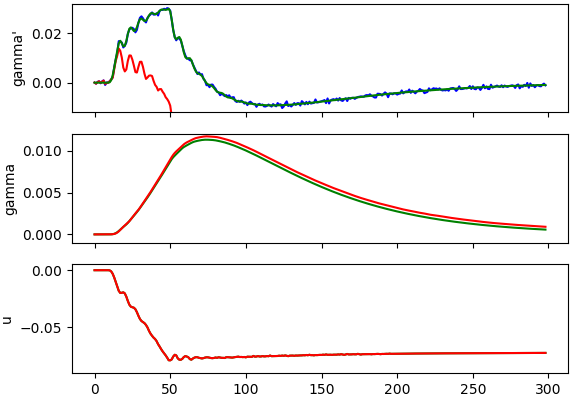
\includegraphics[width=\textwidth]{kalman_attitude_servo_Q0_01_usaved.png}
\caption{Using saved values for $u$} \label{fig:attitude_Q001_usaved}
\end{subfigure}
\begin{subfigure}[t]{0.48\textwidth}
\centering
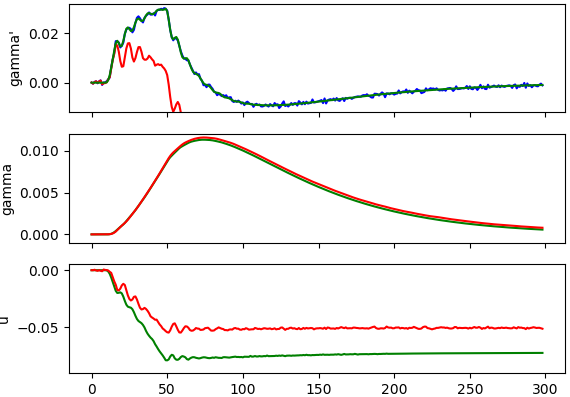
\includegraphics[width=\textwidth]{kalman_attitude_servo_Q0_01_ulive.png} 
\caption{Calculating $u$ from state variables during runtime} \label{fig:attitude_Q001_ulive}
\end{subfigure}
\caption{Estimating the rocket's attitude using a more complex state including the servo angle} \label{fig:attitude_Q001}
\end{figure}

For comparison, the command $u$ was either taken from the simulation or calculated during runtime of \texttt{kal""man\_""atti""tude\_""servo"".py} from the state variable estimates according to the PID controller constants described in section \ref{PID}. Keeping the system error covariance as before at $Q=0.01I$, the path angle estimate diverges slightly, whereas the error on the angular velocity $\dot{\gamma}$ is rather large and, in the case of live calculation of $u$, results in a significant error. The results are shown in figure \ref{fig:attitude_Q001}.

\section{Conclusion}

Attitude estimation yields better results using a simple model only taking the path angle and its derivatives into account and regarding servo input and other ``disturbances'' as process noise. The reasons for this are unclear. Of course the \textsc{scilab} simulation is not exactly reproduced in the Kalman filter implementation, and the simple $X_{i+1} = \begin{pmatrix}1 & \Delta t & 0\end{pmatrix} X_i$ integration will diverge from the original data, which was obtained through integration by more refined methods.

The underlying question, which Kalman filter architecture and which PID controller will be able to successfully control RTVC, could not be answered with sufficient certainty.

\end{document}
